\documentclass[12pt,]{article}
\usepackage{lmodern}
\usepackage{amssymb,amsmath}
\usepackage{ifxetex,ifluatex}
\usepackage{fixltx2e} % provides \textsubscript
\ifnum 0\ifxetex 1\fi\ifluatex 1\fi=0 % if pdftex
  \usepackage[T1]{fontenc}
  \usepackage[utf8]{inputenc}
\else % if luatex or xelatex
  \ifxetex
    \usepackage{mathspec}
  \else
    \usepackage{fontspec}
  \fi
  \defaultfontfeatures{Ligatures=TeX,Scale=MatchLowercase}
\fi
% use upquote if available, for straight quotes in verbatim environments
\IfFileExists{upquote.sty}{\usepackage{upquote}}{}
% use microtype if available
\IfFileExists{microtype.sty}{%
\usepackage{microtype}
\UseMicrotypeSet[protrusion]{basicmath} % disable protrusion for tt fonts
}{}
\usepackage[margin=1in]{geometry}
\usepackage{hyperref}
\PassOptionsToPackage{usenames,dvipsnames}{color} % color is loaded by hyperref
\hypersetup{unicode=true,
            colorlinks=true,
            linkcolor=black,
            citecolor=Blue,
            urlcolor=black,
            breaklinks=true}
\urlstyle{same}  % don't use monospace font for urls
\usepackage{longtable,booktabs}
\usepackage{graphicx,grffile}
\makeatletter
\def\maxwidth{\ifdim\Gin@nat@width>\linewidth\linewidth\else\Gin@nat@width\fi}
\def\maxheight{\ifdim\Gin@nat@height>\textheight\textheight\else\Gin@nat@height\fi}
\makeatother
% Scale images if necessary, so that they will not overflow the page
% margins by default, and it is still possible to overwrite the defaults
% using explicit options in \includegraphics[width, height, ...]{}
\setkeys{Gin}{width=\maxwidth,height=\maxheight,keepaspectratio}
\IfFileExists{parskip.sty}{%
\usepackage{parskip}
}{% else
\setlength{\parindent}{0pt}
\setlength{\parskip}{6pt plus 2pt minus 1pt}
}
\setlength{\emergencystretch}{3em}  % prevent overfull lines
\providecommand{\tightlist}{%
  \setlength{\itemsep}{0pt}\setlength{\parskip}{0pt}}
\setcounter{secnumdepth}{0}
% Redefines (sub)paragraphs to behave more like sections
\ifx\paragraph\undefined\else
\let\oldparagraph\paragraph
\renewcommand{\paragraph}[1]{\oldparagraph{#1}\mbox{}}
\fi
\ifx\subparagraph\undefined\else
\let\oldsubparagraph\subparagraph
\renewcommand{\subparagraph}[1]{\oldsubparagraph{#1}\mbox{}}
\fi

%%% Use protect on footnotes to avoid problems with footnotes in titles
\let\rmarkdownfootnote\footnote%
\def\footnote{\protect\rmarkdownfootnote}

%%% Change title format to be more compact
\usepackage{titling}

% Create subtitle command for use in maketitle
\newcommand{\subtitle}[1]{
  \posttitle{
    \begin{center}\large#1\end{center}
    }
}

\setlength{\droptitle}{-2em}
  \title{}
  \pretitle{\vspace{\droptitle}}
  \posttitle{}
  \author{}
  \preauthor{}\postauthor{}
  \date{}
  \predate{}\postdate{}

\usepackage{lineno}
\usepackage{setspace}
\doublespacing
\usepackage{amsmath}
\usepackage{caption}
\usepackage{bm}
\newcommand{\beginsupplement}{\setcounter{table}{0}\renewcommand{\thetable}{S\arabic{table}}\setcounter{figure}{0}\renewcommand{\thefigure}{S\arabic{figure}}\setcounter{equation}{0}\renewcommand{\theequation}{S\arabic{equation}}}

\begin{document}

\renewcommand*{\thefootnote}{\fnsymbol{footnote}}

\textbackslash{}begin\{titlepage\} \textbackslash{}begin\{centering\}

\sloppy

~

~

~

\textbf{\large{Where do higher order interactions come from?}}

\textbackslash{}textsc\{\small{Andrew R. Kleinhesselink\footnote{Corresponding author: arklein@ucla.edu}\textsuperscript{1}, Jonathan M. Levine\textsuperscript{2}, Nathan Kraft\textsuperscript{1}}

\textit{\small{\textsuperscript{1}Department of Ecology and Evolutionary Biology, University of California, Los Angeles 621 Charles E. Young Drive South Los Angeles, CA 90095 USA}}
\textbackslash{}
\textit{\small{\textsuperscript{2}ETH, Zurich Switzerland}}
\textbackslash{}

\textbackslash{}end\{centering\}

\bigskip \textbf{Running title:} Higher order interactions

\smallskip \textbf{Submission type:} Article \vspace{3 cm}

\renewcommand*{\thefootnote}{\arabic{footnote}}

\setcounter{footnote}{0}

\textbackslash{}end\{titlepage\} \pagebreak{} \linenumbers

\subsection{Abstract}\label{abstract}

In most classical models of species competition, the outcome of
competition is determined by pairwise competition coefficients. However,
almost every community on earth contains many more than two species, and
almost every species interacts with more than one other competitor. It
may be a mistake to assume that models based upon only pairwise per
capita competition adequately describe multi-species communities.

Specifically, higher order interactions (HOI) complicate the use of
pairwise competition coefficients for any community with three or more
species. HOIs occur when pairwise competition coefficients are not fixed
and instead depend on the density of other species in the community. The
question of when and where HOIs occur is thus critical to extending the
insights derived from two species models to natural communities.

In this paper we examine how and when HOIs emerge in simple competition
models when more than two species compete. We break the origin of HOIs
into cases where they result from changes in species densities or sizes
that are not captured in the model structure and cases where they emerge
due to changes in resource use through time.

We conclude that HOIs may be likely to arise when competitors engage in
multiple rounds of competition across the life-cycle. In mechanistic
models, we suggest that HOIs may also emerge when per capita resource
consumption is not fixed, but instead varies over time. Clarifying the
source of HOIs in simple analytical and simulation models may help us
better understand the true nature of competition and the stability of
multispecies communities.

\emph{Key words: competition, coexistence theory}

\subsection{Introduction}\label{introduction}

Almost every species on earth interacts with a vast number of predators,
pathogens and competitors. And the densities of each of these species,
are themselves determined by interactions with yet other species in the
community. Nonetheless, most classical models in community ecology
summarize species interactions with fixed pairwise interaction
coefficients. In particular, pairwise competition coefficients have been
critical to the development of modern coexistence theory (MCT). A
powerful implication arising from the assumption of fixed pairwise
competition coefficients is that the outcome of multi-species species
competition can be predicted by measuring the outcome of competition
between all pairs of species in that community (cite). This assumptions
leads to the idea that a general theory of species competitive exclusion
and coexistence can be achieved if one could simply map pairwise
differences in species' traits and physiology to species pairwise
competition coefficients (Adler et al. 2013, Kraft et al. 2015).

The possibility of higher order interactions (HOIs) between species
challenges the core assumption of pairwise competition coefficients. By
definition, HOIs mean that pairwise competition coefficients are not
themselves fixed, but depend upon the densities of other species in the
community. Among other issues that arise in a world of HOIs are
classical definitions of coexistence and the niche which rely upon
comparing pairwise intraspecific competition coefficients to
interspecific competition coefficients (Chesson, etc. etc.). If HOIs are
common, then predicting community assembly in natural multi-species
communities might not be achieved by measuring all possible pairwise
competitive interactions. Thus, a thorough empirical and theoretical
investigation of HOI in natural communities is critical to expanding
ecological beyond two species models and increasing its relevance in the
natural world.

\paragraph{Defining higher order
interactions}\label{defining-higher-order-interactions}

Despite the potential importance of HOIs in a multi-species world,
competitive HOIs have received relatively little theoretical or
empirical attention. This extends even to the matter of defining what
they are.

To even begin discussing HOIs, we need to first define competition. We
approach the definition from a mechanistic perspective first and then a
phenomenological perspective. From a mechanistic perspective,
competition occurs when individuals consume the same limiting resources.
Increases in consumer densities change the availability of resources
which then changes the growth rate of consumers. Thus at its most basic
resource competition can be thought of as an indirect effect between
individuals mediated by resource concentration. Equivalent models apply
to any limiting environmental factors, such as shared mutualists and
shared predators and pathogens (apparent competition).

In contrast, the phenomenological definition of competition dispenses
with external environmental factors such as resource concentration and
instead focuses on the indirect effects themselves. Phenomenological
competition is measured as the reduction in a per-capita population
growth rate due to an increase in density of individuals of the same
trophic level (cite). This perspective on competition is extremely
powerful because it includes all shared resources and other
environmental feedbacks into one effect that can be measured
empirically. A phenomenological definition of competition also
encompasses direct interactions between individuals of the same trophic
level, such as hemiparisitism, intra-guild predation, interference
competition and allelopathy.

We contrast mechanistic and phenomenological approaches to competition
because they have fundamentally different implications for HOIs. In a
mechanistic model, it is quite hard to define HOIs. If one knows the
resource consumption rates of each species, and the value of those
resources to each species' population growth rate, then you can
calculate the indirect effects of each species on each other and the
stability and trajectory of multi-species communities. HOIs are a
non-issue because they are implicit in the model.

However, in a phenomenological model, the structure and stability of the
community depends on the effects of species densities on other species
population growth rates and in this case HOIs have a clear definition.
In figure 1, competitive effects are depicted as arrows showing that
density of species two reduces the vital rate of species one by some
factor \(\alpha_{12}\). The dashed arrow shows that species three
modifies the competitive effect of species two on one. We take this kind
of interaction modification to be an HOI, specifically a second order
competitive interaction. More generally, pairwise interactions occur
when the effect of species \(j\) on species \(i\) depends only on the
density of species \(j\) and HOIs occur whenever the effect of species
\(j\) on species \(i\) depends also on the density of species other than
\(j\).

\begin{figure}
\centering
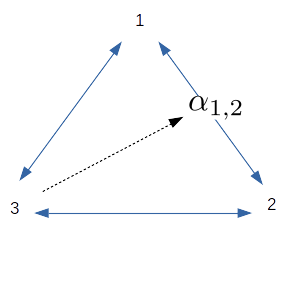
\includegraphics{../figures/HOI_1.png}
\caption{Three species competitive network. Competitive interactions
between species are depicted with the blue arrows. The effect of species
two on one can be described by some function \(\alpha_{12}\). Higher
order interactions occur when the function \(alpha_{12}\) is modified by
the density of another species not involved in the interaction. In this
case, we show a HOI as a dashed line from species three modifying the
effect of two on one.}
\end{figure}

As further illustration of our definition of HOIs we start with a
general model for species phenomenological competition,

\vspace{-1em}

\begin{equation} \label{eq1}
n_{i,t+1} = n_{i,t}f(C), 
\end{equation}

where \(n_{i,t}\) is the density of species \(i\) at time \(t\), \(f\)
is a function that gives the per capita population growth rate as a
function of total competition experienced \(C_i\). Competition between
species \(i\), \(j\) and \(k\) is pairwise and does not involve HOIs if
each species contributes linearly to competition such that
\(C = \sum\alpha_{i,j}(n_j)\), where \(\alpha_{i,j}\) is a function of
competitor density \(n_j\). In contrast, HOIs occur whenever overall
competition \(C\) cannot be broken down into additive pairwise
components.

Consider defining the competition experienced by species 1 as:
\(C_1(n_1,n_2,n_3) = (\alpha_{1,1}n_{1} + \alpha_{1,2}n_{2} + \alpha_{1,3}n_3)\).
If we relax the assumption that pairwise competition coefficients are
fixed and instead allow the competition coefficients to depend on other
competitor densities, our model now includes the possibility of HOIs.
Replace \(\alpha_{1,2}\) with a linear function of \(n_3\),
\(a(n_3) = \alpha_{1,2} + \beta n_3\). Now the competitive effect of
\(n_{2}\) on \(n_{1}\) depends on \(n_3\). The equation for competition
can be re-written as,
\(C_1 = (\alpha_{1,1}n_{1} + \alpha_{1,2}n_{2} + \beta n_{2}n_{3} + \alpha_{1,3}n_{3})\).

In this example, \(\beta\) captures a second order HOI effect of species
\(2\) and \(3\) together. As long as \(\beta \neq 0\) we can no longer
isolate the pairwise effect of species \(2\) or \(3\) on species \(1\).
In general, more diverse communities allow for HOIs of greater order,
with a community of \(s\) species having HOIs of the order \(s-1\)
possible. From an empirical perspective, the presence of HOIs means that
if we measure the per capita population growth rate of each focal
species \(i\) when it is rare (\(n_i \approx 0\)), and we vary the
density of each of the competitors (including \(i\) itself), this will
not be enough to predict the dynamics in a three, or even a two species
community!

Now that we have defined HOIs, we explore a variety of mechanistic and
phenomenological models in order to try and classify the origin of HOIs.
Finally we evaluate whether any of the examples are likely to generate
HOIs in nature.

\subsection{HOIs arrising from cycles of pairwise
competition}\label{hois-arrising-from-cycles-of-pairwise-competition}

HOIs could arise in discrete time models when the time step involves
aggregating of a sequence of pairwise competition events. In a recent
theoretical analysis, Grilli et al. (2017) provided a concise
demonstration of this effect. In their model, seedling trees compete to
fill a forest gap. If competition for the gap occurs as a sequence of
competitive rounds between pairs of individuals then HOIs naturally
emerge. This counter intuitive result occurs because the probability
that a species wins the gap depends not only on its direct pairwise
interactions, but also on the pairwise interactions between its
competitors. In effect, which competitor the species interacts with in
round two of the tournament depends on those competitors interactions in
round one. Because of these indirect effects, we cannot express the gap
filling tournament with a single set of pairwise competition
coefficients, we need to include HOIs in the model.

In the Grilli model, competition involved a tournament of discrete
winner-take-all competitive events. The idea of having plant competition
occur one at a time may perhaps seem unrealistic. However, their model
captures a general process that could apply to many types of models. As
another example we consider an annual plant population that follows a
two stage model. Seeds germinate and survive into adults with
probability \(p\): \(a = n_{t}p\), where \(a\) is adult density at an
intermediate time within the growing season, and \(n_{t}\) is the
initial seed density at the time \(t\). After that, adults produce the
next generation of seeds via a fecundity rate \(f\): \(n_{t+1} = af\).
Because the plants are annuals there is no adult survival.

We can introduce competition by making fecundity of species \(i\) a
function of adult density of all species in the community:
\(f_i = f_i(a_i, a_j)\). Seedling germination and survival could also be
function of competition, so we could make \(p_i\) a function of initial
seed density such that \(p_i = p_i(n_i, n_j)\).

Now we consider a two species community with initial seed densities for
species one and two of \(n_1\) and \(n_2\) and calculate the per capita
seed production of species 1 over the time step \(t\) to \(t+1\),

\vspace{-1em}

\begin{equation} \label{eq2}
\frac{n_{1,t+1}}{n_{1,t}} = p_1( n_{1,t}, n_{2,t} )f_1( a_{1,u}, a_{2,u} ) 
\end{equation}

In the model above, adult density is an intermediate state variable that
is both the product of competition during the first part of the growing
season but also contributes to competition during the reproductive
phase. Re-writing to eliminate the intermediate phase,

\vspace{-1em}

\begin{equation} \label{eq3}
\frac{n_{1,t+1}}{n_{1,t}} = p_1( n_{1,t}, n_{2,t} )f_1( n_{1,t}p_1( n_{1,t}, n_{2,t} ), n_{2,t}p_2( n_{1,t}, n_{2,t} ) ) 
\end{equation}

This equation shows that the effect of two on one cannot be fully
captured by pairwise effects. It also depends on the initial density of
one and how strongly one reduces the survival of two. This is apparent
when considering the arguments to the fecundity function \(f_i\)
contains the density of both competitors multiplied by their survival
functions.

Aggregating the survival and reproduction phases of the life-cycle and
the competitive effects on each, results in a complicated equation
involving numerous polynomial terms of \(n_{1,t}\) and \(n_{2,t}\) and
HOI terms.

One way of interpreting the above model is to consider it a case where
there is a distinct survival niche and a distinct fecundity niche. The
survival niche is encoded by the matrix \(\alpha_ij\) whereas the
fecundity niche is encoded by \(\beta_ij\). Most plant populations
encompass some kind of stage structure and it seems likely that
competitive effects between individuals probably vary depending on the
stage structure.\\
\emph{I'd like to do some more work on this. I think having an example
where we show how HOIs emerge analytically. Specifically if we could
show analytically how the two stages of competition given by the
\(\alpha\) and \(\beta\) in a two stage lifecycle model contribute to
HOIs that would be really useful. My hunch is that HOI terms cancel out
in some circumstances which is why we can successfully model populations
without HOI terms in a lot of cases. The problem is that the expression
for HOIs will depend very much on how we account for competition in the
two lifestage transitions. Unfortunately, I wasted a lot of time trying
to analyze the above and have become a bit stuck!}

\subsection{HOIs in a mechanistic resource competition
model}\label{hois-in-a-mechanistic-resource-competition-model}

Unlike the phenomenological model above, we can also imagine HOIs
emerging from mechanistic models.

Because experimental data evaluating HOIs at the demographic level is
lacking, we developed a mechanistic simulation of annual plant
competition for a single shared resource. We then try and describe
competition in the system using a simple phenomenological competition
model.

\paragraph{Resource mechanistic model}\label{resource-mechanistic-model}

Our mechanistic model is inspired by California annual plant communities
growing in a Mediterranean climate. In this environment, rainfall starts
in the winter and gradually declines through the spring while
temperature and evaporative demand increase. Plants germinate in the
winter and begin to flower in spring. By summer, most plants have
completed flowering and produce seeds and die. In our model we track a
single pool of generic soil resources, perhaps water or mobile inorganic
nutrients. The resource supply rate spikes in early spring and then goes
to zero as the spring progresses. Thus the pool of resources is
exemplified by non-equilibrium pulse dynamics and never reaches an
equilibrium.

In our model, rates of plant growth depend on resource availability. As
spring progresses, plants grow larger but resource supply diminishes.
Eventually plants reach a point where their resource uptake rates cannot
keep up with respiration and maintenance costs. At this point, we assume
that plants stop producing vegetative biomass and start producing seeds.
We simplify this by assuming that all biomass is converted to seed
biomass at a fixed rate instantaneously. At this point the adult plants
die and stop taking up resources.

The model is expressed as a set of differential equations,

\vspace{-1em}

\begin{equation} \label{eq4}
\frac{dR}{dt} = S(t) - \sum_{i = 1}^sB_{i}f(R,r, K)
\end{equation}

where \(R(t)\) gives the resource availability at time \(t\), and \(S\)
gives the resource supply rate at time \(t\). The final term expresses
the loss of resources due to uptake by plants. We sum over each of the
\(s\) species in the community to get total uptake. Annual plant biomass
of species \(i\) at time \(t\) is given by \(B\) and the uptake rate is
a function \(f_i\) of total resource availability. We simulate a
Mediterranean climate by setting initial resource availaibility high
setting the resource supply rate \(S(t)\) to zero.

Growth of each species depends on resource availability,

\vspace{-1em}

\begin{equation} \label{eq5}
\frac{dB_{i}}{dt} = B_{i}(qf_i(R) - m)
\end{equation}

Where, \(B_i\) is the total biomass of species \(i\), \(q\) is a
resource conversion factor, \(m\) is a per biomass respiration and
tissue loss rate, and as in the first equation, \(f_i\) is the resource
uptake rate.

In this model, the growth of each species stops when \(qf_i(R) = m\)
meaning that biomass gained is equal to biomass lost to respiration and
maintenance. Because the summer drought will only further reduce
resource concentrations, the optimal behavior of the plant at this point
is to stop growing and convert stored resources to seed mass. We impose
this behavior on the model by setting biomass at time \(z\) (\(B(z)\))
to zero when \(m\) matches resource uptake and conversion:
\(qf_i(R(z)) = m\).

Different species are likely to have different rates of resource uptake,
respiration and tissue loss rates. In our simulations we assume a
trade-off between rates of resource uptake at high resource availability
and rates of resource uptake at low resource availability. This means
that species which dominate early in the season when resource
availability is high will stop growing earlier in the season as resource
availibility declines. In contrast, species that grow slower early in
the growing season are able to persist later into the season when
resource availability is low.

We enforce this trade-off between species by giving each species \(i\) a
unique resource uptake function \(f_i\) that depends on two species
specific parameters \(r_i\) and \(K_i\),

\vspace{-1em}

\begin{equation} \label{eq7}
f_i(R, r_i, K_i) = r_iR/(K_i + R)
\end{equation}

Example resource uptake curves for a fast growing early season species,
a mid season species, and a slower growing late season species (resource
uptake fig).

\begin{figure}
\centering
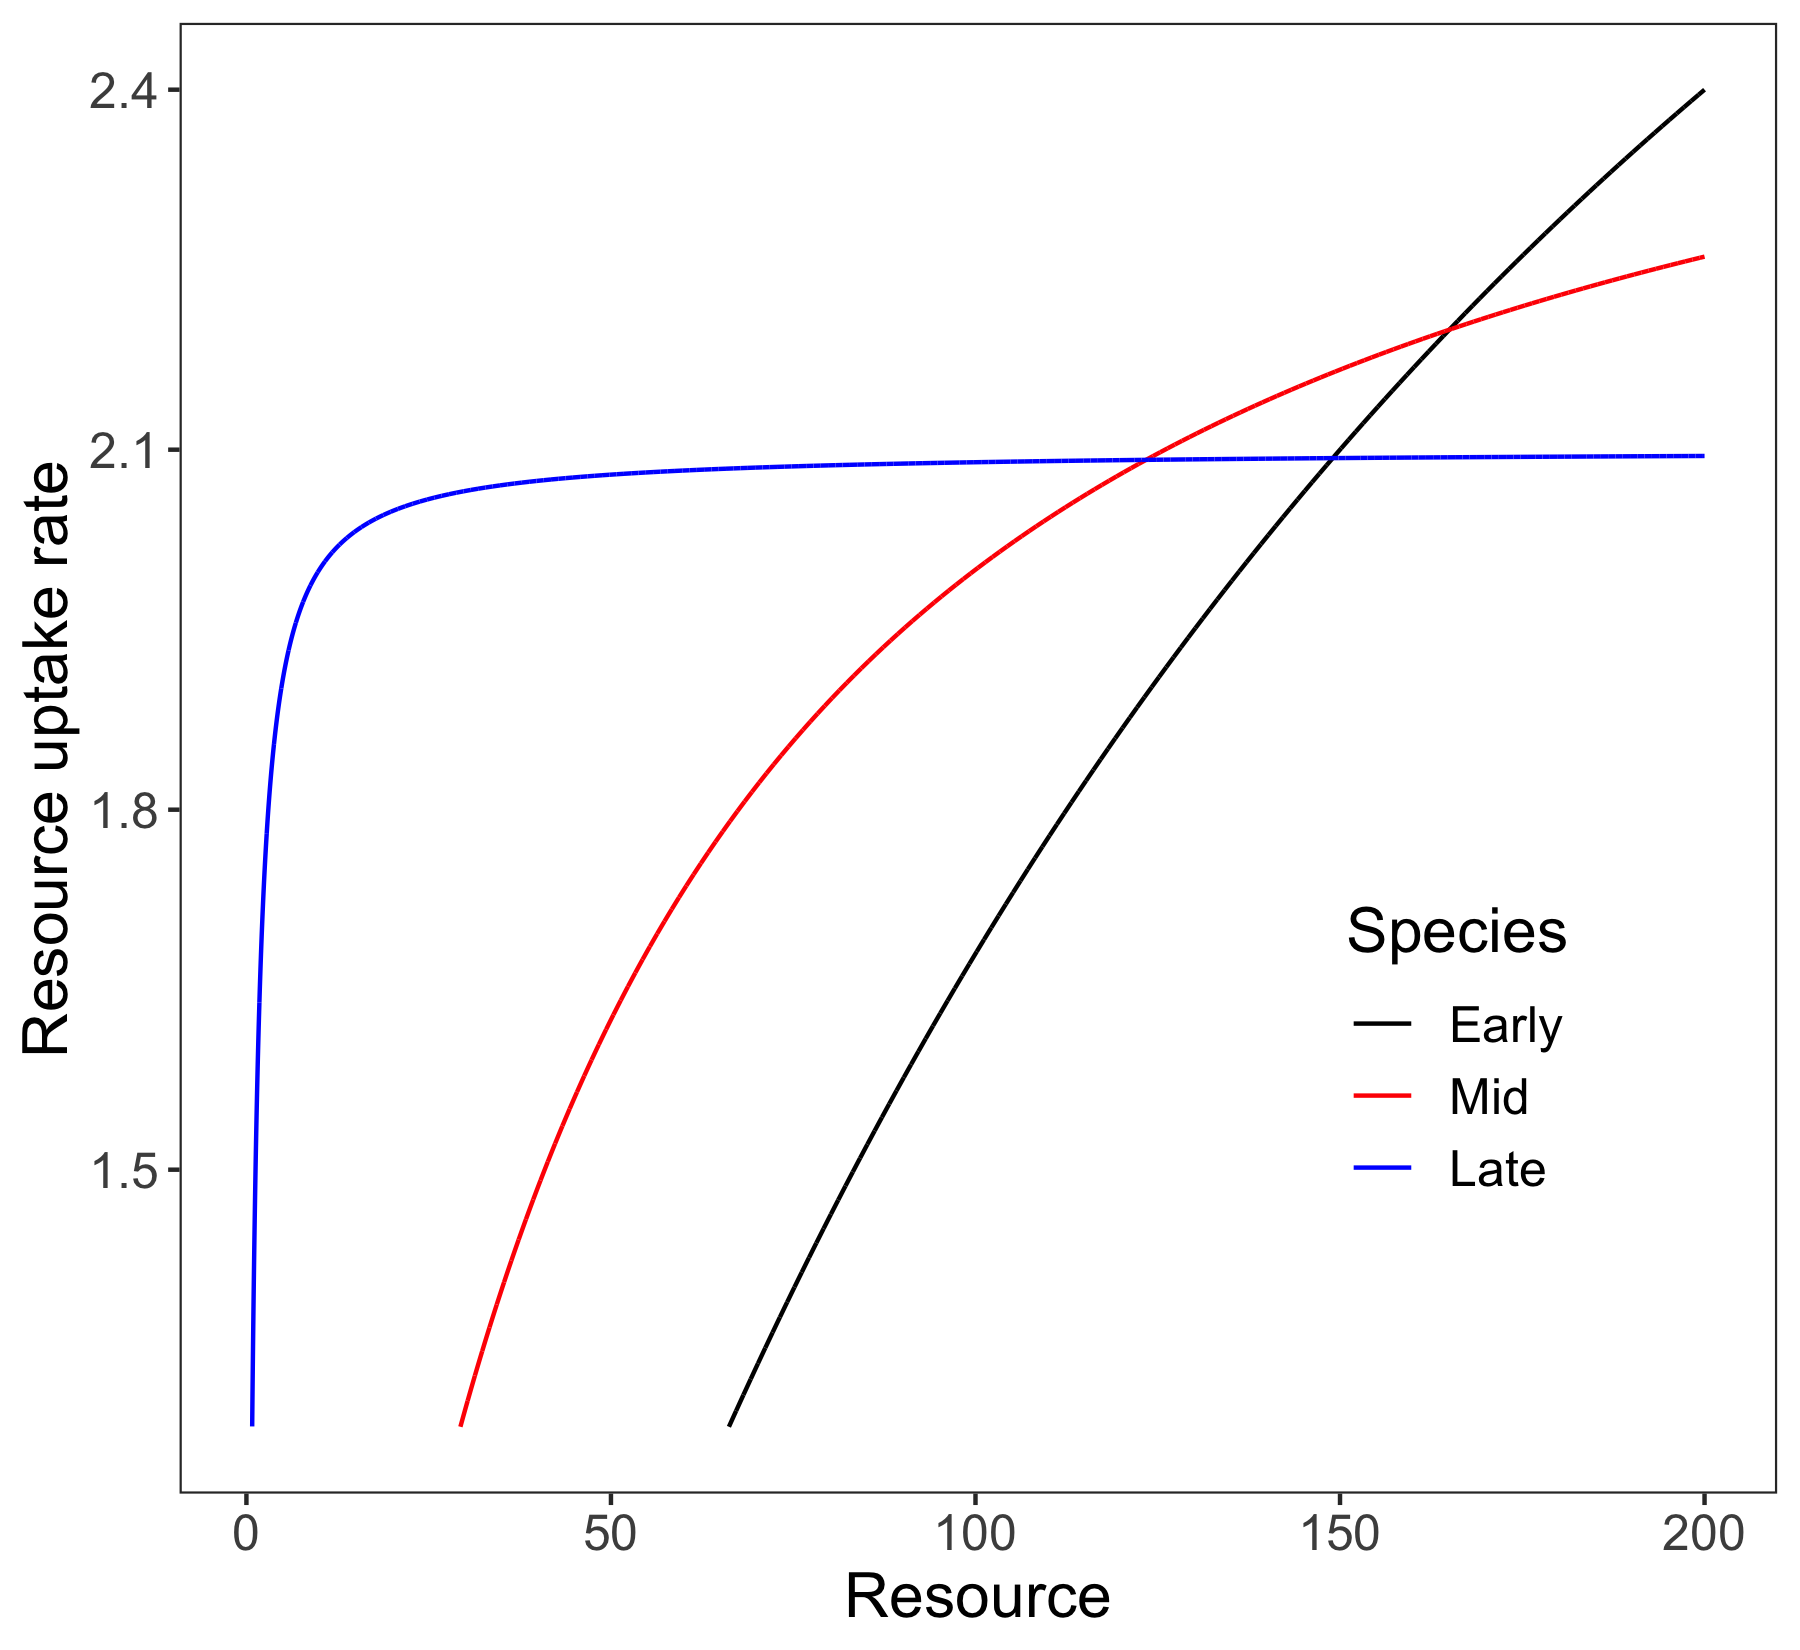
\includegraphics{../figures/resource_uptake.png}
\caption{Resource curves for three simulated species. Species one has a
resource uptake advantage when resource availability is high whereas
species three has a resource uptake advantage when resource availability
is low.}
\end{figure}

The unique resource uptake curves for species one and two result in
species one growing faster earlier in the season but also flowering and
senescing earlier. Species two grows slower early in the season but is
able to grow later into the season (growth phenology fig).

\begin{figure}
\centering
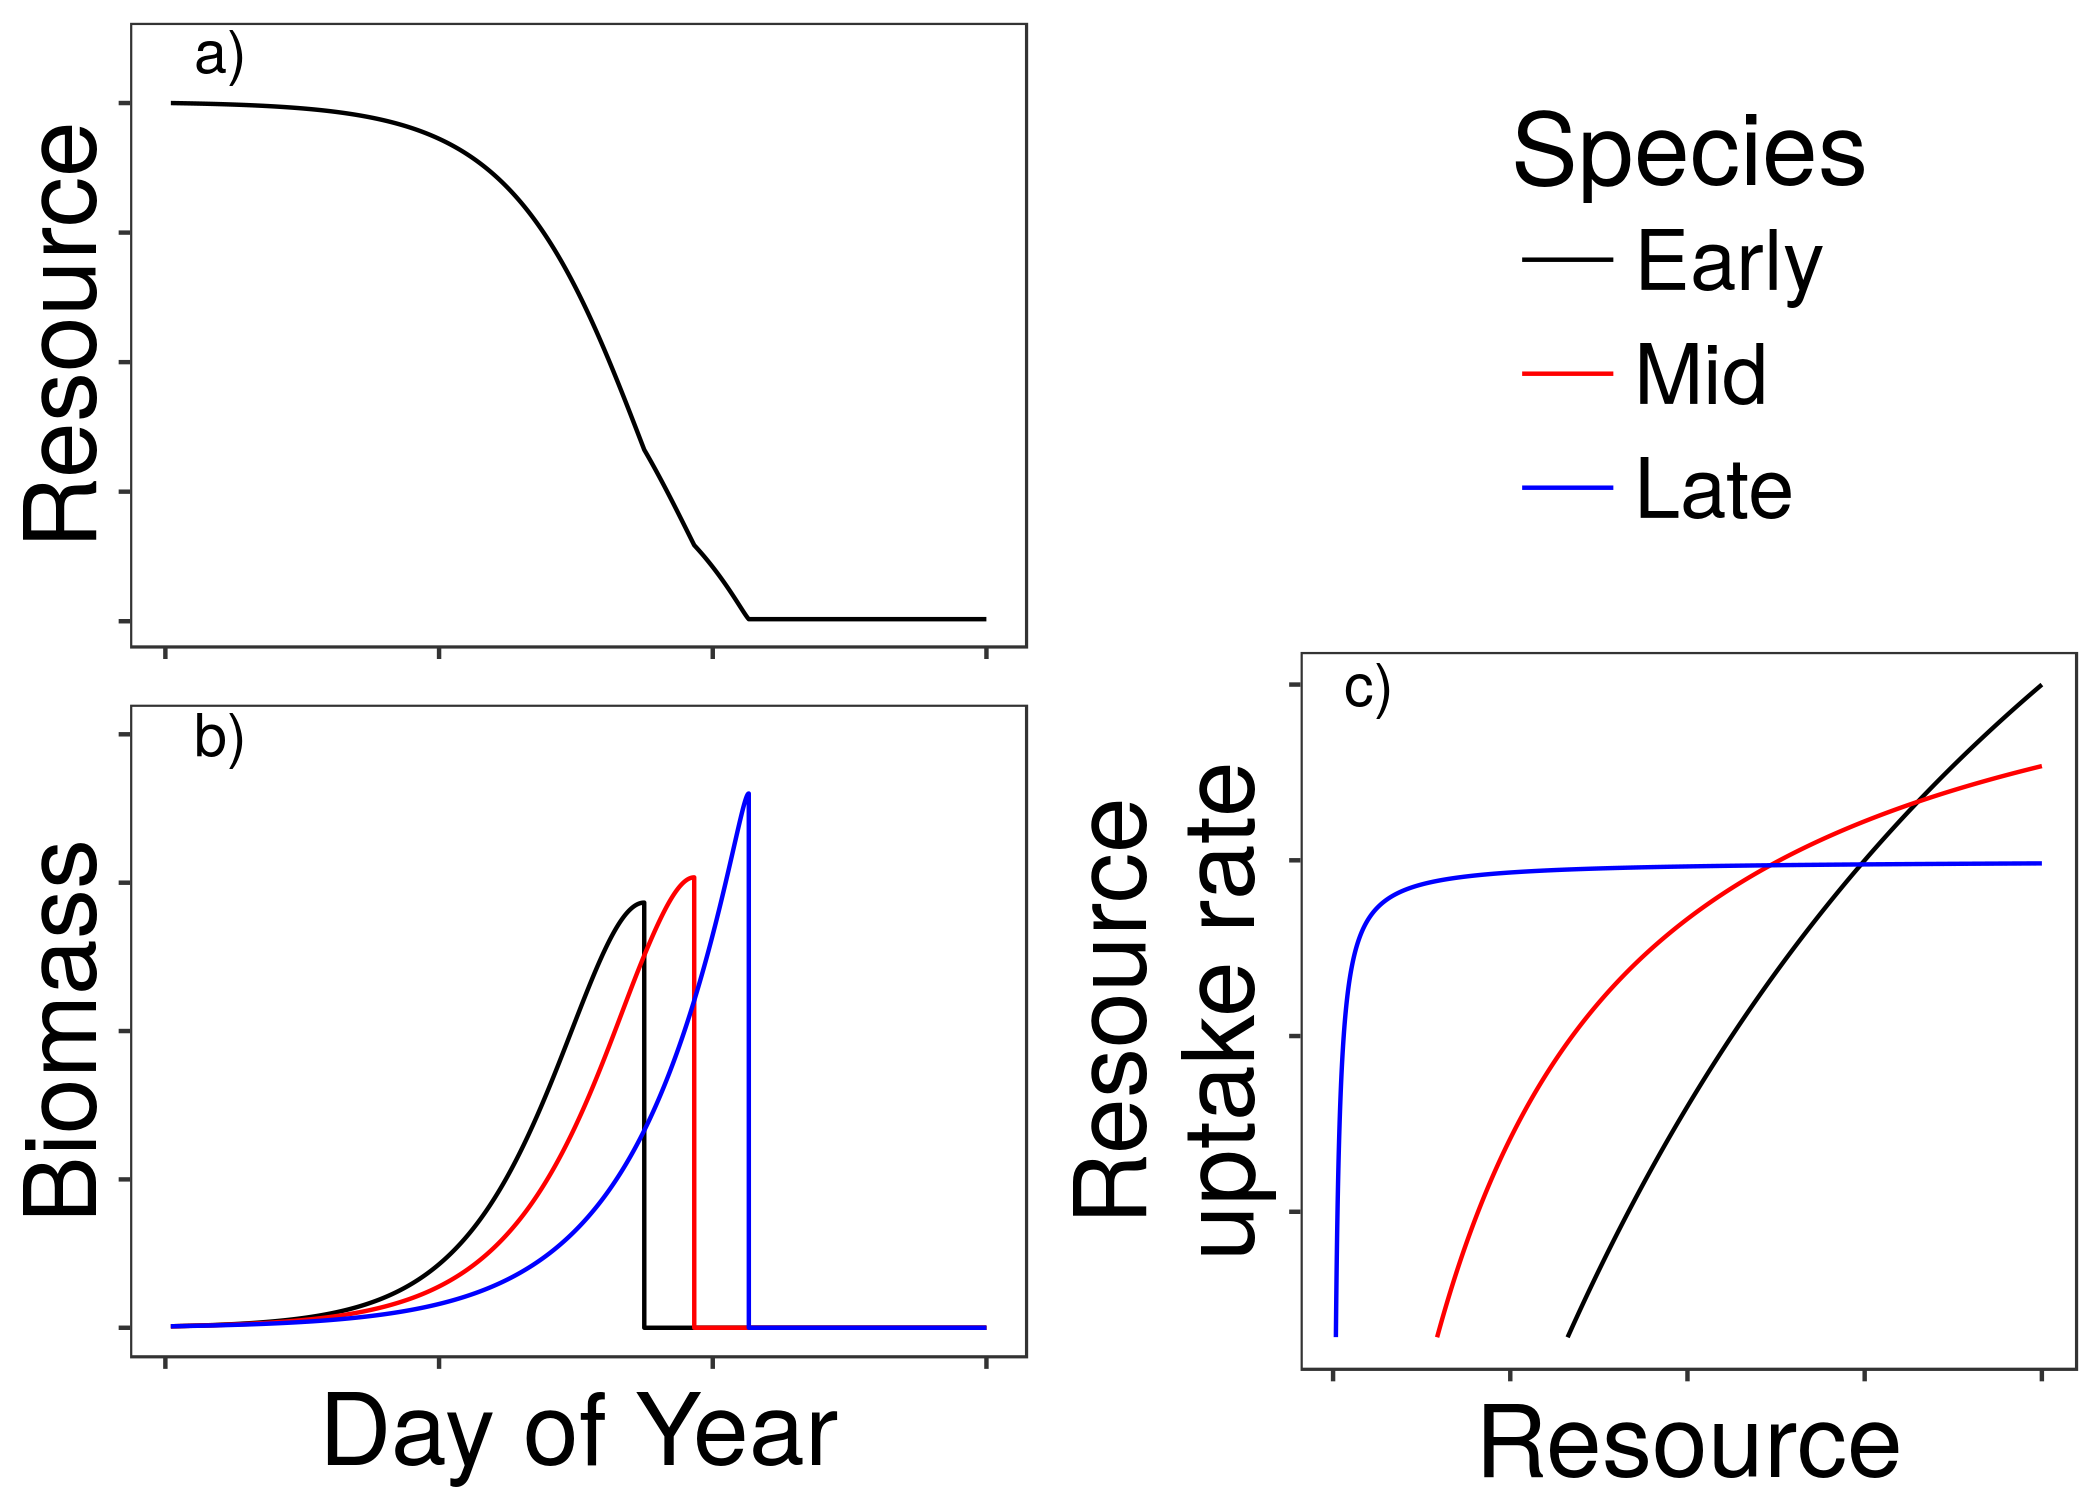
\includegraphics{../figures/example_timeseries.png}
\caption{Example time series showing draw down of the resource during
the course of the simulation, upper panel, and growth of each of the
species, lower panel. Species one grows rapidly early in the season, but
senesces early as well. Species three grows slowly early in the season
but grows for a longer period of time. Species is somewhere between
these extremes. Each species reaches its peak biomass at a different
time, at which point we assume all vegetative biomass is converted to
seed mass, and resource uptake by that species stops.}
\end{figure}

So far we have described a model run in continuous time within a single
generation. For this model we denote rates of change of biomass and
resources within the season in terms of very small time intervals \(t\).
By contrast, we keep track of total population size of each generation
at a discrete annual time scale \(\tau\). To calculate the total
population size of each species at time step \(tau+1\) we take each
species' maximum vegetative biomass during the growing season, multiply
that by a conversion factor \(c\) to get a seed mass, and then multiply
that by a constant seed per gram ratio, \(\mu\). Thus,

\vspace{-1em}

\begin{equation} \label{eq6}
n_{i,\tau+1} = \mu c(\max B_i)_{\tau}, 
\end{equation}

where \(n_{i,\tau+1}\) is the number of seeds produced. To simplify the
interpretation of the model, we assume that there is no seed mortality
between years and all seeds germinate.

We simulate these dynamics using the ordinary differential equation
solvers package \(\tt{desolve}\) in the statistical program R.
Simulation parameters and code to run the simulations are given in the
supporting information.

\paragraph{Response surface
experiment}\label{response-surface-experiment}

Using the model described above we simulated a response surface
experiment where individuals of each of the three species are grown
against increasing densities of inter- or intraspecific competitors. We
then calculate the per capita reproductive output of the focal species
and fit phenomenological competition models to our simulated data. We
only include simulations in which the focal species faces fewer than
three competitor species at once.

\paragraph{Phenomenological annual plant
model}\label{phenomenological-annual-plant-model}

We model annual plant competition in terms of the decline in per capita
reproductive output with increasing density of competitors at the start
of the growing season (\(n_{j,tau}\)). We use a standard functional form
for phenomenological competition that has been used a number empirical
studies of annual plant competition (Kraft et al. 2015),

\vspace{-1em}

\begin{equation} \label{eqBeverton}
\frac{ n_{i,\tau+1} }{ n_{i,\tau} } = \lambda_{i}/(1 + \sum^3_{j=1} \alpha_{i,j} n_{j,\tau})^{ \eta_i } ,
\end{equation}

where \(\eta_{i} > 0\) and \(\lambda_i > 0\). In this model,
\(\lambda_i\) denotes maximum per capita reproductive output,
\(\alpha_{ij}\) is the per capita competitive effect of species \(j\) on
\(i\) and \(\eta_i\) is a species specific parameter controlling the how
steep fecundity declines with competition in general. We refer to this
functional form as the basic model.

In order to assess the importance of HOIs, we can include various higher
order terms in the basic functional form. In the case of three species,
this includes three pairwise effects, three quadratic effects and three
second order HOI terms,

\vspace{-1em}

\begin{equation} \label{eqHOI}
\frac{ n_{i,\tau+1} }{ n_{i,\tau} } = \lambda_{i}/(1 + \sum^3_{j=1} \alpha_{i,j} n_{j,\tau} + \sum^3_{j=1}\gamma_{i,j}n_j^2 + \beta_{i,1}n_1n_2 + \beta_{i,2}n_1n_3 + \beta_{i,3}n_2n_3)^{ \eta_i },
\end{equation}

We refer to this competition model as the HOI model. We fit each of
these competition models using the \(\tt{nls}\) function in the
statistical language R. We calculate \(\lambda_{i}\) for each species as
the per capita fecundity in the absence of any competitors, and set this
as a fixed parameter in the model.

\paragraph{Model fits}\label{model-fits}

The basic Beverton-Holt functional form (eq.) is a good fit for the
effects of both inter and intraspecific competition on species one and
adding HOI terms does not qualitatively improve model fit (fig below).

\begin{figure}
\centering
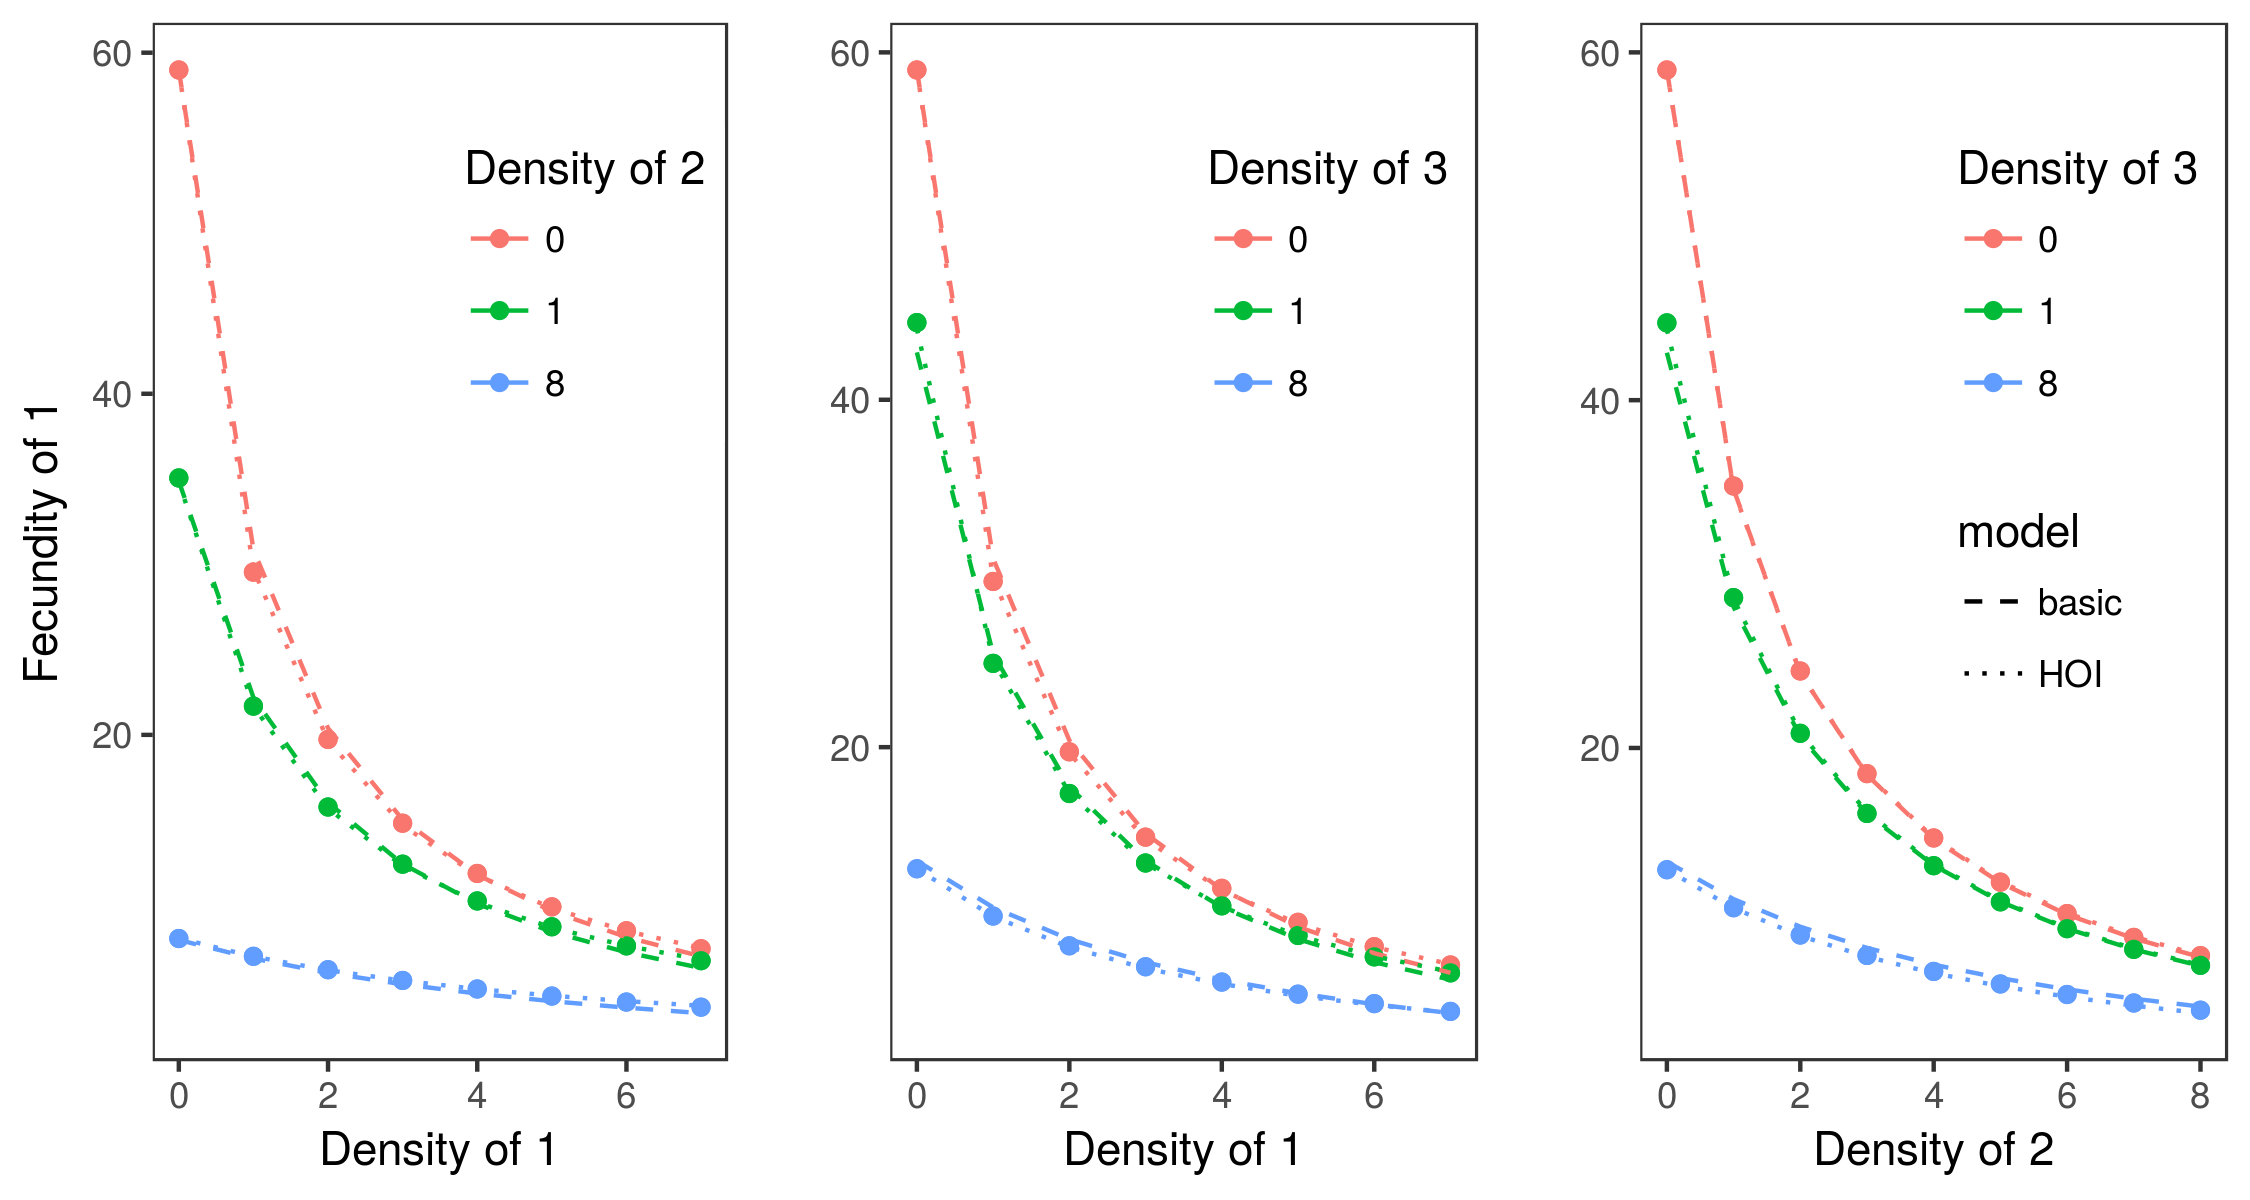
\includegraphics{../figures/species_1_fits_three_species.png}
\caption{Simulated per capita seed production of species one in response
to increasing competitor density on the x-axis. Colored lines show three
different levels of density of a second competitor. The dashed line
shows the best fit line from the basic model and the dotted line shows
the best fit from the HOI model}
\end{figure}

For species two we see more of a discrepancy between the basic and HOI
model fits ( fig below). This is especially apparent in the third panel
which shows the interaction between the densities of species one and
species three. The basic model tends to underpredict the impact of
species one and two together on species two.

\begin{figure}
\centering
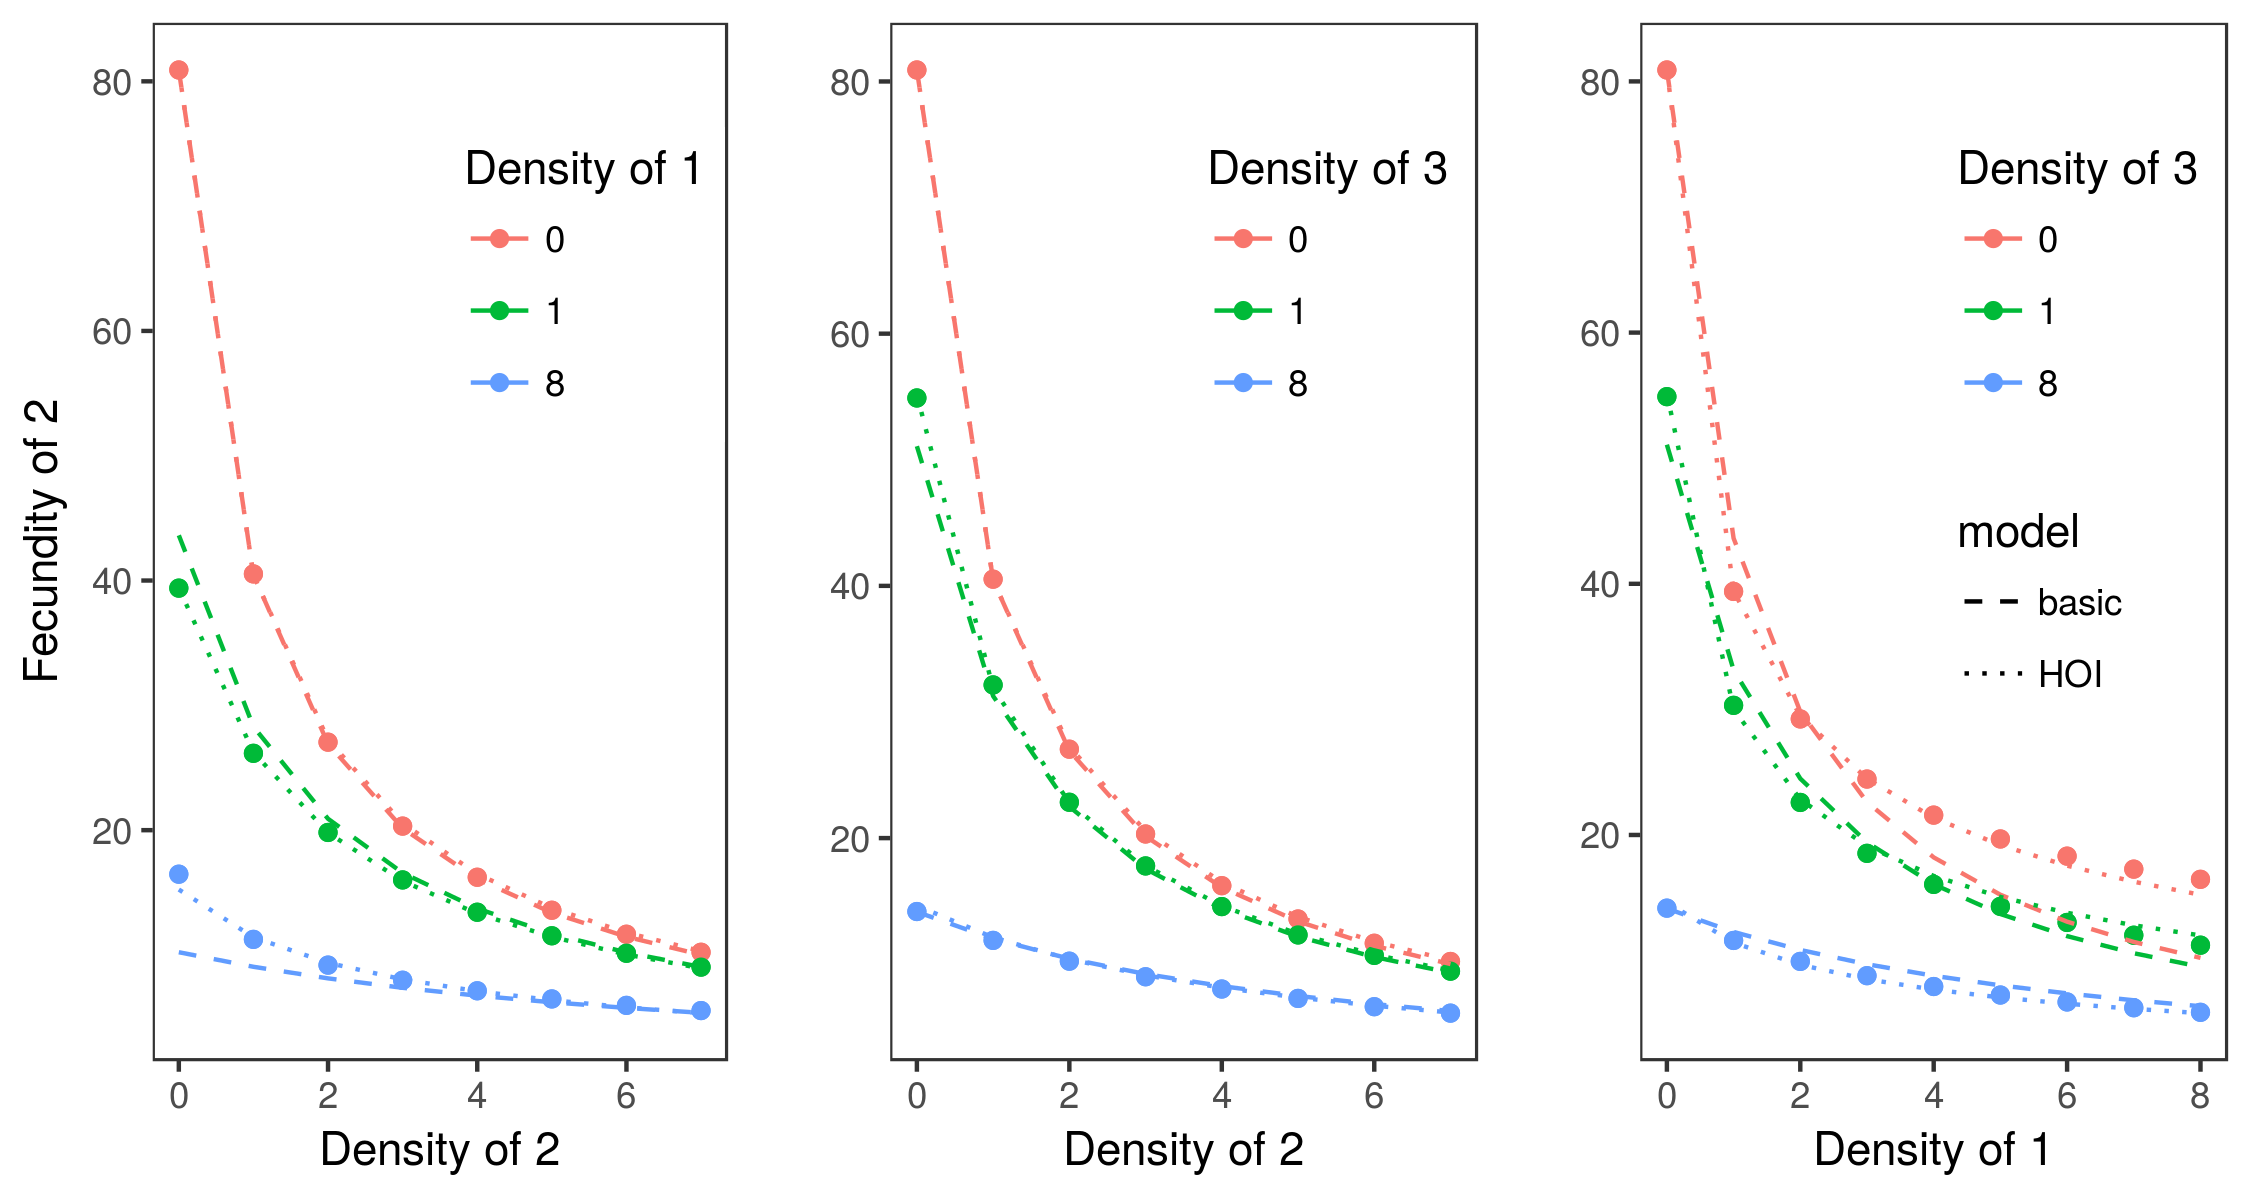
\includegraphics{../figures/species_2_fits_three_species.png}
\caption{Simulated per capita seed production of species two in response
to increasing competitor density on the x-axis. Colored lines show three
different levels of density of a second competitor. The dashed line
shows the best fit line from the basic model and the dotted line shows
the best fit from the HOI model}
\end{figure}

Finally, for species three, we see an even greater discrepancy between
the basic and HOI model fits (fig below). This is apparent in all three
panels. The HOI fit appears to be quite good in the first two panels.
The HOI fit appears to be least accurate at high densities of species
one and low densities of species two (rightmost panel).

\begin{figure}
\centering
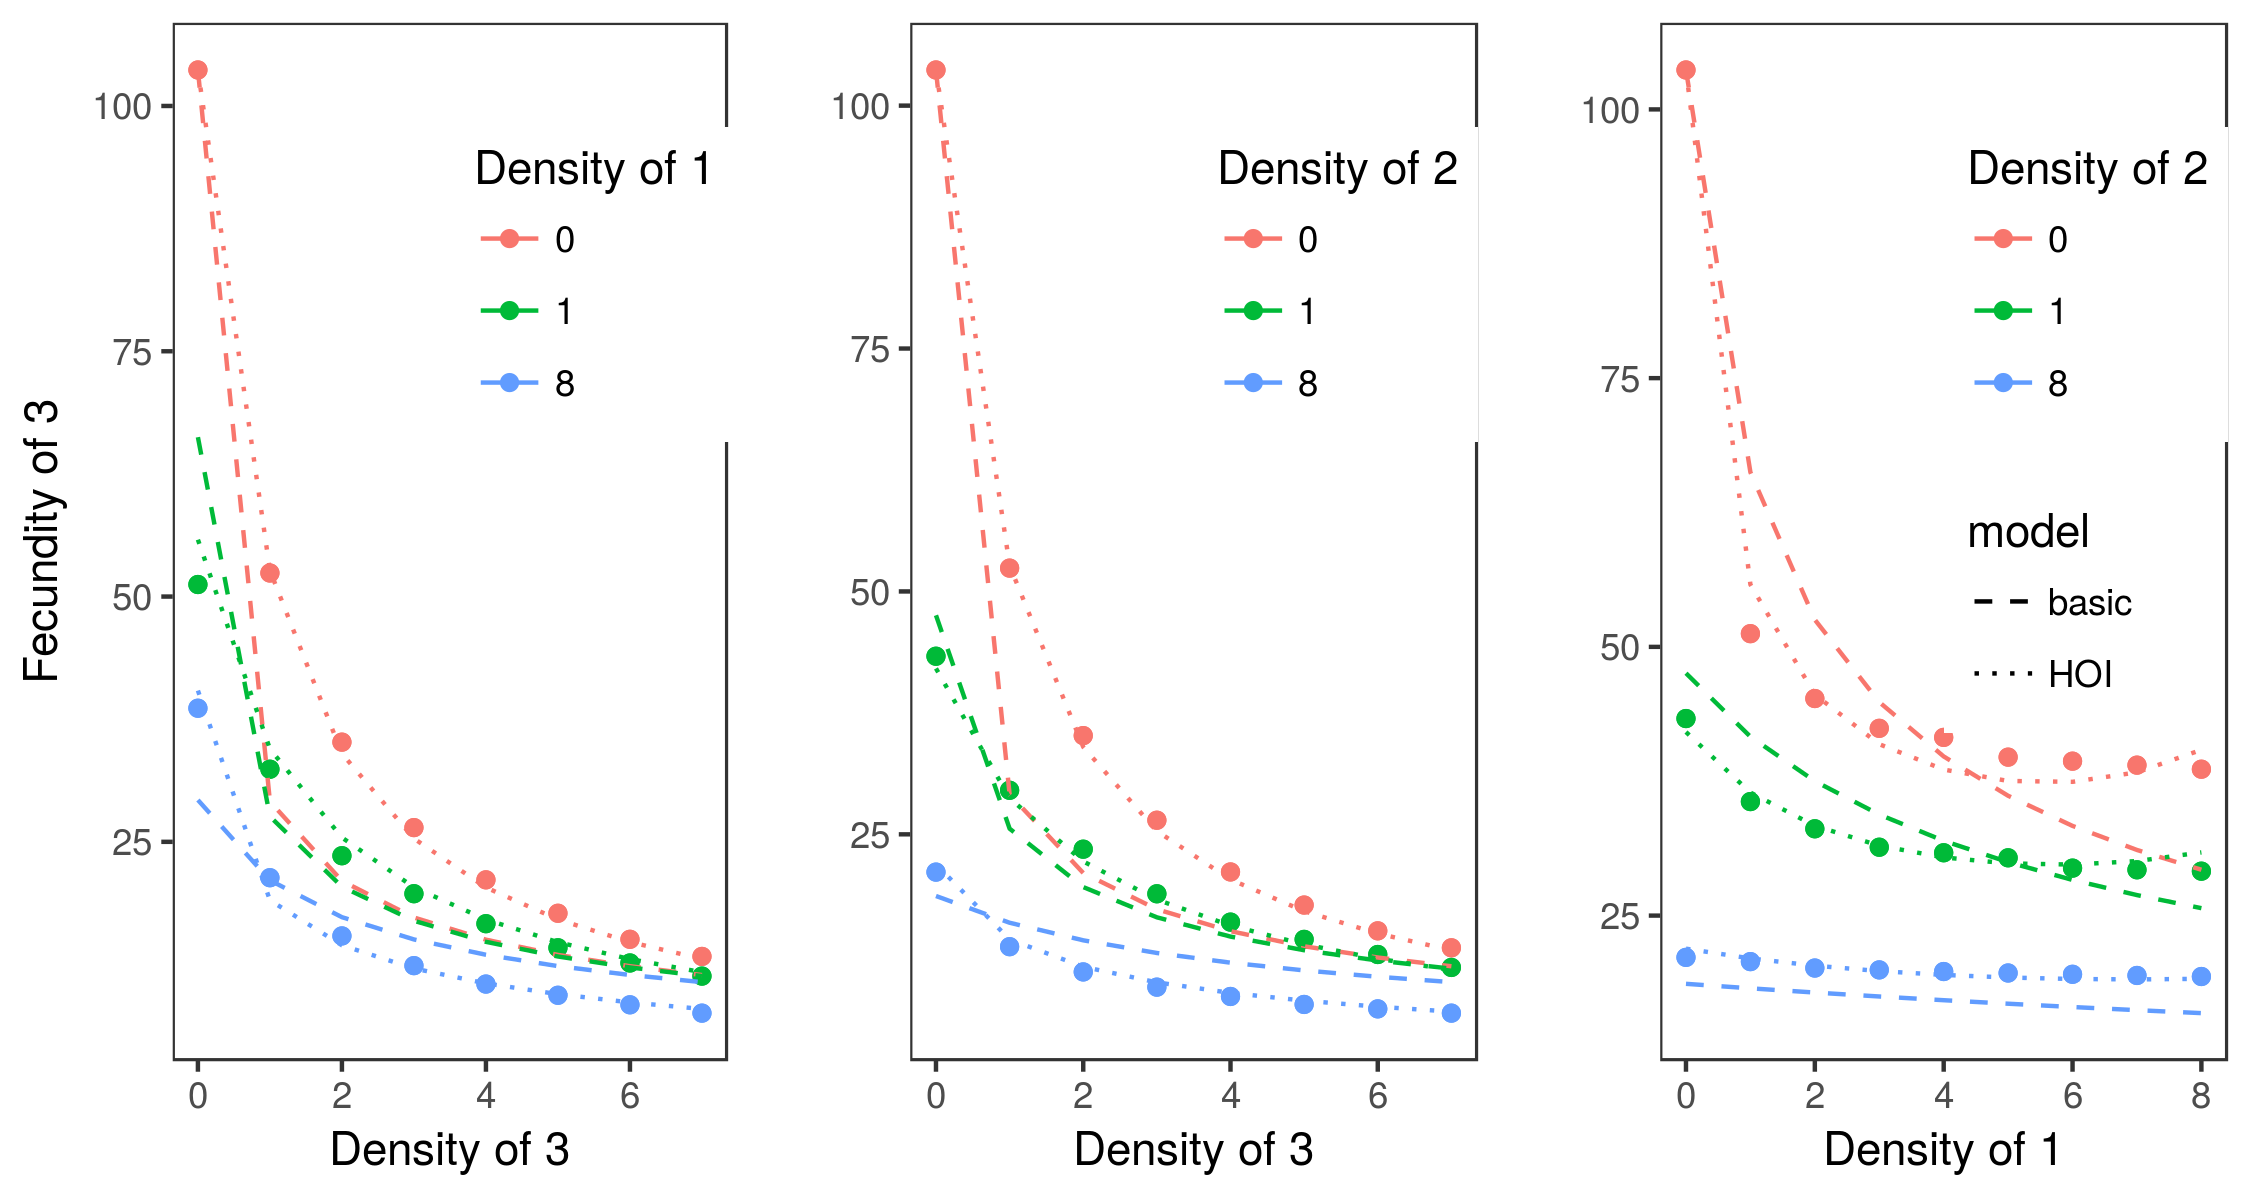
\includegraphics{../figures/species_3_fits_three_species.png}
\caption{Simulated per capita seed production of species three in
response to increasing competitor density on the x-axis. Colored lines
show three different levels of density of a second competitor. The
dashed line shows the best fit line from the basic model and the dotted
line shows the best fit from the HOI model}
\end{figure}

For each of the three species, including HOI and quadratic terms
improves model fit in terms of residual squared error (table below). For
species one, the quadratic and HOI terms are small relative to the
pairwise effects. For species two and three, the HOI terms are of
similar magnitude to the pairwise effects, in some cases stronger.

\begin{longtable}[]{@{}llrrrrrrrrrr@{}}
\caption{Fitted HOI parameters and residiual squared error for the basic
model and the model containing higher order interaction
terms}\tabularnewline
\toprule
species & model & \(N_1\) & \(N_2\) & \(N_3\) & \(N_1^2\) & \(N_2^2\) &
\(N_3^2\) & \(N_1N_2\) & \(N_1N_3\) & \(N_2N_3\) & error\tabularnewline
\midrule
\endfirsthead
\toprule
species & model & \(N_1\) & \(N_2\) & \(N_3\) & \(N_1^2\) & \(N_2^2\) &
\(N_3^2\) & \(N_1N_2\) & \(N_1N_3\) & \(N_2N_3\) & error\tabularnewline
\midrule
\endhead
1 & basic & 0.74 & 0.57 & 0.32 & - & - & - & - & - & - &
0.33\tabularnewline
1 & HOI & 0.83 & 0.58 & 0.28 & -0.02 & 0.00 & 0.01 & -0.01 & 0.00 & 0.01
& 0.08\tabularnewline
2 & basic & 0.84 & 0.98 & 0.58 & - & - & - & - & - & - &
1.19\tabularnewline
2 & HOI & 2.97 & 2.03 & 0.78 & 0.00 & 0.74 & 0.30 & 1.91 & 1.64 & 1.09 &
0.28\tabularnewline
3 & basic & 1.46 & 3.78 & 11.78 & - & - & - & - & - & - &
3.41\tabularnewline
3 & HOI & 3.69 & 7.89 & 1.43 & -0.33 & -0.38 & 2.57 & 0.11 & 5.33 & 8.60
& 0.76\tabularnewline
\bottomrule
\end{longtable}

\paragraph{Interpreting the fits}\label{interpreting-the-fits}

It is clear from the above example that a relatively simple resource
consumption model may require HOI terms in order to be fit by a
phenomenological model. The obvious question is how to interpret these
additional quadratic and second order HOI terms. On the one hand it
should not be surprising that adding additional terms improves model
fit. Many functions can be approximated to an arbitrary level of
precision by a power series. We essentially are approximating a power
series by summing over polynomial terms of ever increasing order.

However, in this case we believe the HOI effects play a more meaningful
role than simply helping us approximate an completely unknown function.
In support of this argument, we note that the basic Beverton-Holt model
does an adequate job fitting the response of species one to the
competitive effects of one and two. It is only for species two and three
that we begin see evidence of important HOI effects.

We believe this has to do with the temporal nature of competition in
this system. While species one is active, species two and three are also
always active. Thus the effects of intitial competitor density on
species one are relatively simple. Increasing densities of competitors
will supress the resource capture by species one and thus change its
overall performance in a constant manner regardless of the mix of
species.

However, for species two and three the competitive environment is more
complex. For example, take species two competing only against species
one. The growing season can be split up into two phases: the first part
of the growing season over which species two interacts with species one
and itself; and the second part of the growing season where species two
only interacts with itself. Working backwords from the time when species
two flowers, we might be able to predict its ultimate size and fecundity
from its biomass at the time that species one stops growing. That part
of the growing season only involves intraspecific competition so it
should be relatively simple. But the intraspecific competition
experienced by species two over this second part of the growing season
depends on how large it is at the start of this second phase of growth.
So we have to predict its size at the start of phase two. This in turn,
depends on the inter- and intraspecific competition experienced over the
first phase of the growing season.

Keeping this in mind we can rationalize the HOI terms for species two as
describing the inter- and intraspecific effects of competitor density on
species two during the first phase of the growing season, multiplied by
only the intraspecific over the second phase of the growing season. For
species two this leads to a strong effect of intraspecific densities
squared, and an effect of interspecific density multiplied by
intraspecific density (table above). Noticably absent is a quadratic
effect on the density of species one, which makes sense given this
interpretation (table).

Likewise there is an HOI term for the effects of species one and three
acting together on species two. Once again, we need to consider the two
phases of competition experienced by species two. First the density of
species one and three will determine the biomass of species three when
species one flowers. This will then determine the interspecific effects
of species three on two during the second phase of the growing season
for species two. Thus we see a strong effect of species three's density
squared and a strong HOI between the intial density of species three and
species one.

The competitive dynamics for species three are even more complex. This
late season species goes through three distinct phases of competition,
first competing with all three species, then only with two and then
finally with only itself. Working backwards from its final bimoass and
reproductive output, species three's performance will depend on its size
when species two flowers, which will depend on the size of two and three
when species one flowers, which will depend on the inital densities of
all three species. Because there are effectively three cycles of
competitor density and response to consider for species three its
reasonable to expect that third order HOI terms resolve some of the lack
of fit observed for this species (see figure ).

This system is characterized by a seasonal pulse of resource
availability and the lack of an equilibrium between species biomass and
resource concentrations in the environment. In contrast, if resources
were supplied continually, at some level \(S\), then eventually species
biomass would increase until resource uptake matched this level of
resource supply. This is a classic result from mechanistic resource
modeling (chemostat papers, Tilman etc.). At this equilibrium, the
sensitivity of each species to the densities of each other species can
be approximated with a linear phenomenological model (cite Meszena,
Kleinhesselink, Tilman). This focus on the equilibrium dynamics, and an
avoidance of the messiness inherent in periodically forced
non-equilibrium systems may be one reason HOI's have received little
attention among competing species.

\subsection{Discussion}\label{discussion}

\subsection{Conclusions/Summary (?? )}\label{conclusionssummary}

We have sought to clarify the definition of HOI's and explain how they
could arise from relatively simple competitive dynamics. We illustrate
this point with two hypothetical models of species competition. In the
first model, simple pairwise interactions iterated over multiple life
stages could lead to HOI's. In the second, we show that a community
characterized by pulses of resource supply and sequential cycles of
species competition and senescence could also lead to HOI's. A general
theme in both models, is that HOI's arise when the competitive
environment and species abundances change at a time step shorter than
the interval over which the effects of competition are observed. As
researchers begin to focus their efforts on detecting HOIs, it seems
likely that HOI's will increasingly be found among competiting species.

\subsection{Acknowledgments}\label{acknowledgments}

\pagebreak{}

\subsection{References}\label{references}

\setlength{\parindent}{-0.2in} \setlength{\leftskip}{0.2in}
\setlength{\parskip}{12pt} \noindent

\hypertarget{refs}{}
\hypertarget{ref-adler_trait-based_2013}{}
Adler, P. B., A. Fajardo, A. R. Kleinhesselink, and N. J. B. Kraft.
2013. Trait-based tests of coexistence mechanisms. Ecology Letters
16:1294--1306.

\hypertarget{ref-kraft_plant_2015}{}
Kraft, N. J. B., O. Godoy, and J. M. Levine. 2015. Plant functional
traits and the multidimensional nature of species coexistence.
Proceedings of the National Academy of Sciences of the United States of
America 112:797--802.

\pagebreak{}

\setlength{\parindent}{0in} \setlength{\leftskip}{0in}
\setlength{\parskip}{12pt}

\subsection{Tables}\label{tables}

\pagebreak{}

\subsection{Figure Legends}\label{figure-legends}

\textbf{Figure \ref{fig:hypothesis}.}

\textbf{Figure \ref{fig:map}.}

\textbf{Figure \ref{fig:effects}.}

\pagebreak{}

\subsection{Figures}\label{figures}

\pagebreak{}

\section{Appendix S1:}\label{appendix-s1}

\beginsupplement

\subsection{Mechanistic Model}\label{mechanistic-model}

\pagebreak{}

\subsection{Tables}\label{tables-1}

\pagebreak{}

\subsection{Figures}\label{figures-1}


\end{document}
